\documentclass{beamer}
\usepackage{listings}
\lstset{
%language=C,
frame=single, 
breaklines=true,
columns=fullflexible
}
\usepackage{subcaption}
\usepackage{url}
\usepackage{tikz}
\usepackage{graphicx}
\usepackage{tkz-euclide} % loads  TikZ and tkz-base
%\usetkzobj{all}
\usetikzlibrary{calc,math}
\usepackage{float}
\newcommand\norm[1]{\left\lVert#1\right\rVert}
\renewcommand{\vec}[1]{\mathbf{#1}}
\newcommand{\R}{\mathbb{R}}
\newcommand{\C}{\mathbb{C}}
\providecommand{\brak}[1]{\ensuremath{\left(#1\right)}}
\providecommand{\abs}[1]{\vert#1\vert}
\providecommand{\fourier}{\overset{\mathcal{F}}{ \rightleftharpoons}}
\providecommand{\sbrak}[1]{\ensuremath{{}\left[#1\right]}}
\usepackage[export]{adjustbox}
\usepackage[utf8]{inputenc}
\usepackage{amsmath}
\usetheme{Boadilla}
\title{My Presentation}
\author{Adepu Adarsh Sai}
\institute{IITH(AI)}
\date{\today}
\begin{document}

\begin{frame}
\titlepage
\end{frame}
\begin{frame}{Fourier Transforms}
%\frametitle{Fourier Transforms}
There are several common conventions for defining the Fourier transform of an integrable function $f:\R \rightarrow \C$.One of them is
\begin{align}
    F(t)=\int_{-\infty}^{\infty}f(x)e^{-i2\pi xt}dx
\end{align}
and the inverse Fourier transform of F is 
\begin{align}
    f(x)=\int_{-\infty}^{\infty}F(t)e^{i2\pi xt}dt
\end{align}
\end{frame}
\begin{frame}{Theorem}
Let $g:\R \rightarrow \C$ and $G:\R \rightarrow \C$ be two functions such that
\begin{align}
     g\brak{x} &\fourier G\brak{t}\\
     \implies G\brak{t} &\fourier g\brak{-x} \label{th}
\end{align}
where $ \fourier$ represents Fourier transform and
\begin{align}
    G\brak{t}  = \int_{-\infty}^{\infty} g\brak{x} e^{-i2\pi xt} dx 
    \label{F}
\end{align}
\end{frame}
\begin{frame}{Proof}
\begin{align}
    g(x)=\int_{-\infty}^{\infty}G(t)e^{i2\pi xt}dt
\end{align}
changing $x \rightarrow -x$
\begin{align}
    g(-x)=\int_{-\infty}^{\infty}G(t)e^{-i2\pi xt}dt
\end{align}
Comparing with \eqref{F}
\begin{align}
    \implies G\brak{t} &\fourier g\brak{-x} \label{th1}
\end{align}
\end{frame}

\begin{frame}{Some Useful Functions}
\begin{block}{Rectangular Function}
\begin{align}
 rect\brak{\frac{x}{\tau}}=
\begin{cases}
1 & ,\frac{-\tau}{2} < x < \frac{\tau}{2}\\
\frac{1}{2}& ,\abs{x}=\frac{\tau}{2}\\
0 & ,otherwise
\end{cases} 
\end{align}
\end{block}
\begin{block}{Sinc function}

\begin{align}
Sinc(x)&=
\begin{cases}
1 & x=0\\
\frac{\sin{\pi x}}{\pi x} & otherwise
\end{cases}
\end{align}
\end{block}
\end{frame}
\begin{frame}{Figures}
\begin{figure}[!ht]
\centering
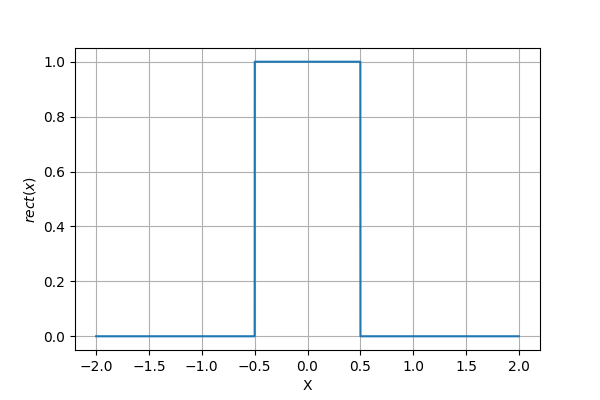
\includegraphics[width=\columnwidth]{rect.png}
\caption{$rect(x)$}
\label{rect}
\end{figure}
\end{frame}
\begin{frame}{Figures}
\begin{figure}[!ht]
\centering
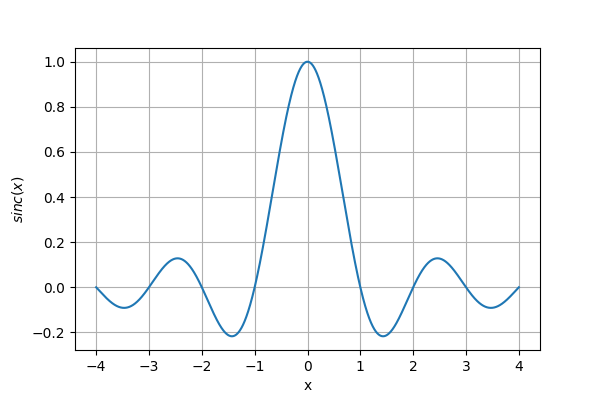
\includegraphics[width=\columnwidth]{sinc.png}
\caption{$sinc(x)$}
\label{rect}
\end{figure}
\end{frame}
\begin{frame}{Fourier transform of rectangular function}
\begin{align}
    \int_{-\infty}^{\infty} rect\brak{\frac{x}{\tau}} e^{-i2\pi xt} dx&= \int_{\frac{-\tau}{2}}^{\frac{\tau}{2}} e^{-i2\pi xt}dx\\
    &=\sbrak{\frac{e^{-i2\pi xt}}{-i2\pi t}}_{\frac{-\tau}{2}}^{\frac{\tau}{2}}\\
    &=\frac{e^{-i\pi t\tau}-e^{i\pi t\tau}}{-i2\pi t}\\
    &=\tau \frac{\sin{\pi t\tau}}{\pi t\tau}\\
    &=\tau sinc(t\tau)
\end{align} 
So
\begin{align}
     rect\brak{\frac{x}{\tau}} &\fourier \tau sinc(t\tau)
\end{align}
\end{frame}
\begin{frame}{Question}
\begin{block}{(GATE 2020(ST) Q16)}
The characteristic function of a random variable X is given by
\begin{align}
\phi_{X}\brak{t}
=
\begin{cases}
\frac{\sin{t}\cos{t}}{t}           & t \neq 0 \\
1        & t = 0
\end{cases}
\end{align}
Then $ P\brak{|X|\leq \frac{3}{2}} =$ 
\end{block}    
\end{frame}
\begin{frame}{Solution}
 The characteristic function of a random variable is defined as
 \begin{align}
     \phi_{X}(t) = \int_{-\infty}^{\infty} f_{X}(x)e^{itx}dx
     \label{ch}
 \end{align}
 where $f_{X}(x)$ is pdf of X.\\
eq\eqref{ch} is one of the conventions of Fourier transform.So $\phi_{X}(t)$ is Fourier transform of $f_{X}(x)$.From Inversion Theorem
\begin{align}
    \implies f_{X}(x)=\frac{1}{2\pi} \int_{-\infty}^{\infty}  \phi_{X}\brak{t}e^{-ixt} dt 
\end{align}
\end{frame}
\begin{frame}{Solution}
   We know that 
   \begin{align}
    rect\brak{\frac{x}{\tau}} &\fourier \tau sinc(t\tau)
\end{align}
from \eqref{th} we have
\begin{align}
  \tau sinc(t\tau) &\fourier rect\brak{-\frac{x}{\tau}}\\
   \implies rect\brak{-\frac{x}{\tau}} &= \int_{-\infty}^{\infty} \tau \frac{\sin{\pi t \tau}}{{\pi t \tau}} e^{-i2\pi xt}dt
\end{align}
substituting $\tau = \frac{2}{\pi}$ and changing $2\pi x \rightarrow x $ we get
\begin{align}
    \frac{1}{4}rect\brak{\frac{-x}{4}} = \frac{1}{2\pi} \int_{-\infty}^{\infty} \brak {\frac{\sin{2t}}{2t}}e^{-jxt} dt
    \label{f}
\end{align}
\end{frame}

\begin{frame}{Solution}
From \eqref{f} the pdf is given by
  \begin{align}
    f_{X}(x) = \frac{1}{4}rect\brak{\frac{-x}{4}} dx
\end{align}
So
\begin{align}
     P\brak{|X|\leq \frac{3}{2}}&=\int_{-\frac{3}{2}}^{\frac{3}{2}} \frac{1}{4}rect\brak{\frac{-x}{4}}dx \\
      &=\int_{\frac{-3}{2}}^{\frac{3}{2}} \frac{1}{4} dx\\
    &=\frac{3}{4}
\end{align}
\end{frame}
\end{document}